\chapter{Theory}
\label{chap:Theory}
%
\section{Statistical Mechanics}
First we consider the system of the crystal of Neon Atoms as a canonical ensemble, this means it will be described under the assumption of an infinitely large heat bath by Boltzmann statistics. The probability distribution of members of the ensemble will then be 
\begin{align}
	p(\vec{\mathbf{q}},\vec{\mathbf{p}})=\frac{e^{-\beta H(\vec{\mathbf{q}},\vec{\mathbf{p}})}}{\int\cdots\int e^{-\beta H(\vec{\mathbf{q}},\vec{\mathbf{p}})}\mathrm{d}^{3N}\vec{\mathbf{q}}\mathrm{d}^{3N}\vec{\mathbf{p}}},
\end{align}
with $N$ being the number of particles.\\\\
Now an ensemble is to be understood as many fictional copies of the same system representing the states that a system will explore when propagating in time according to Hamilton's equation of motion. The ensemble distribution represents the relative number of times that an ergodic system will come by a given state after an infinite amount of time has passed. Now for a crystal in principle this still holds. At low temperatures though the phase space that is being explored can be abstracted in such cases. The reason is that the system will for a given finite time usually explore only nearby points in the phase space. This is the crystal configuration but allowing for dynamics such as lattice vibrations and thermal movement of the atoms with respect to their lattice site. So for a given initial point in phase space the system will mostly explore its proximity until it probabilistically jumps to another volume of phase space whose proximity then will be explored for some further time. Now this means the systems lattice configuration has changed which at low but non zero temperature should be reasonable. 
We now consider these volumes of phase space (being approximately confined regions, i.e. configurations of e.g. a crystalline structure) to be discrete states that the system can be in. So our canonical distribution now is a discrete one, each state representing such a configuration volume. What's left is to figure out what state of the still continuously possible states inside will be used to represent each configuration. We in this work will use the state $(\vec{\mathbf{q}}_{0i},\vec{\mathbf{p}}_{0i})$ that locally minimizes $H(\vec{\mathbf{q}},\vec{\mathbf{p}})$. Such a minimum can be found by employing a relaxation calculation in \ac{LAMMPS}. The Boltzmann distribution now follows to be:
\begin{align}
	p(\vec{\mathbf{q}}_{0i},\vec{\mathbf{p}}_{0i})=\frac{e^{-\beta H(\vec{\mathbf{q}}_{0i},\vec{\mathbf{p}}_{0i})}}{\sum_{n} e^{-\beta H(\vec{\mathbf{q}}_{0n},\vec{\mathbf{p}}_{0n})}}.
\end{align}

\begin{figure}
	\centering
	%trim = left bottom right top
	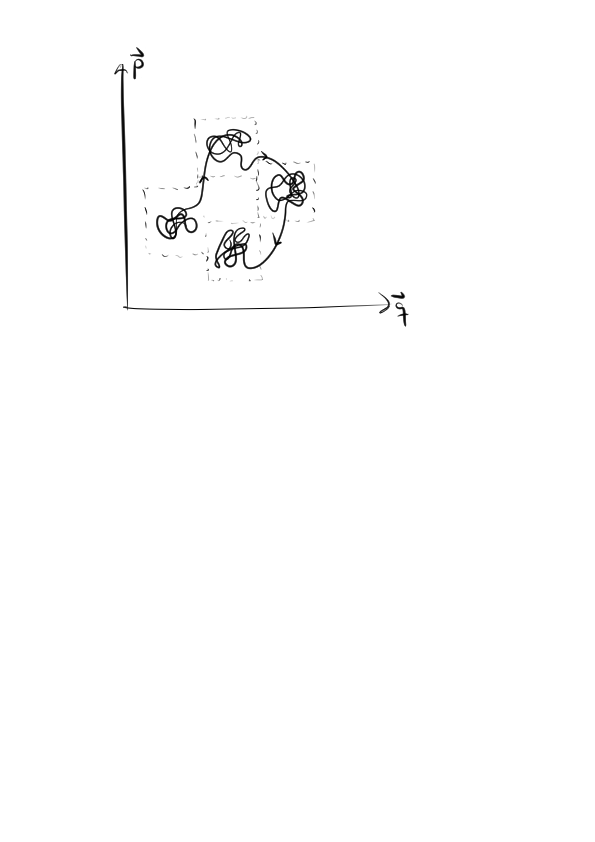
\includegraphics[trim=3cm 18cm 6cm 1.5cm, clip,scale=0.7]{./Inhalt/Bilder/phasespace.png}
	\caption{state evolution $(\vec{\mathbf{q}}(t),\vec{\mathbf{p}}(t))$ through 6N-dimensional phase space}
	\label{fig:phasepsace}
\end{figure}

grand canonical ensemble with two chemical components

sub term of grand canonical ensemble with only ne1 and ne2

Explanation for cohesive energy
\section{Relaxation in LAMMPS}
relaxation theory form lammps 
described in \cite{Bitzek2006} Bitzek, Koskinen, Gahler, Moseler, Gumbsch, Phys Rev Lett, 97, 170201 (2006).
Testcite Griffiths\cite{griffithsQM}
 
\section{Simulated Annealing}
The object that is being annealed is a state vector containing binary information for every lattice site. It refers to the ideal static lattice of the neon structure. A positive value or 1 refers to an atom being present in the initial structure and a negative value or 0 means the neon atom is vacant at this site. So every digit of the binary state refers to a certain specific lattice site. The energy functional of the annealing process will be the energy after minimization (i.e. relaxation) of the above described state vector. This state vector therefore refers to an initial pre-relaxation configuration where sites are simply removed with \ac{LAMMPS}.

Energy functional contains cohesive Energy/chemical potential, not just hamiltonian!!
\lstinputlisting[
float=htpb,
language=Python,
label=lst:simannealing,
caption={Simulated annealing algorithm},]
{Inhalt/Code/code_simulatedannealing.txt}

\section{Symmetry optimization} 
In the case of a single sodium atom inserted in the neon crystal the highly symmetrical structure was exploited to reduce redundant minimization calls in the annealing routine, by identifying symmetrically equivalent structures and caching them. Applying rotation and reflection matrices of the octahedral symmetry group to a single configuration was used to quickly create all equivalent configurations. By sorting them lexicographically and picking e.g. the first, one ensures every redundant set of configurations is always represented by the same configuration.

\lstinputlisting[
float=htpb,
language=Python,
label=lst:ohsorting,
caption={lexicographically sorting point group symmetries},]
{Inhalt/Code/code_lexicographcialsorting.txt} 

\section{DFT optical spectra}






%